\documentclass[11pt]{scrartcl}

\usepackage{ucs}
\usepackage[utf8x]{inputenc}
\usepackage{ngerman}
\usepackage{amsmath,amssymb,amstext}
\usepackage{graphicx}
\usepackage[automark]{scrpage2}
\usepackage{pgfplots}
\usepackage{chngcntr}
\counterwithin{figure}{section}

\pagestyle{scrheadings}

\title{Implementation des ADT Set}
\author{Finn Jannsen, Philipp Schwarz}
\date{\today{}}

\begin{document}

\maketitle

\tableofcontents

\section{Einführung}
\label{sec:einfuehrung}

Diese Dokumentation beschreibt drei Implementations-Varianten des Abstrakten Datentyps Set. Dieser Datentyp soll eine Menge darstellen.
Als Vorgabe zur Art der Implementation wurde 1. ein Array von Elementen, 2. ein Array von Containern und 3. eine verkettete Liste von Containern angeführt.
In Abschnitt \ref{sec:implementation} wird darauf eingegangen, wie die verschiedenen Varianten realisiert wurden.
Anschließend wird in Abschnitt \ref{sec:verfun} geprüft, ob die vorgegebenen Operationen funktionieren und in Abschnitt \ref{sec:aufwand} die Performance der Varianten verglichen.

\section{Implementation}
\label{sec:implementation}

Die drei Varianten wurden in Java als Klassen implementiert. Da alle den gleichen Funktionssatz brauchen implementieren sie alle das gleiche Interface namens SetInterface.\\
Abbildung \ref{figure:classdia} stellt die verwendeten Klassen und Interfaces dar. Dort ist auch zu sehen, welche Methoden das SetInterface vorgibt. Für Interkompatibilität bezüglich der Vereinigung von Mengen wurde die unify-Methode statisch gemacht. Die jeweiligen Implementationen sind bezüglich unify(s1, s2) interkompatibel, da sie jegliche Sets, die das SetInterface implementieren entgegennehmen und dieses zu einem neuen Set (Typ abh. von aufgerufener Methode) vereinigen.\\
Auch wurden Maßnahmen gegen Verstöße, vor allem das verwenden von Pos-Objekten aus uneigenen Sets, getroffen.\\
Mittels Generics wurden Elem und Pos außerdem kompatibel zu allen drei Varianten modelliert.

\begin{figure}[h!]
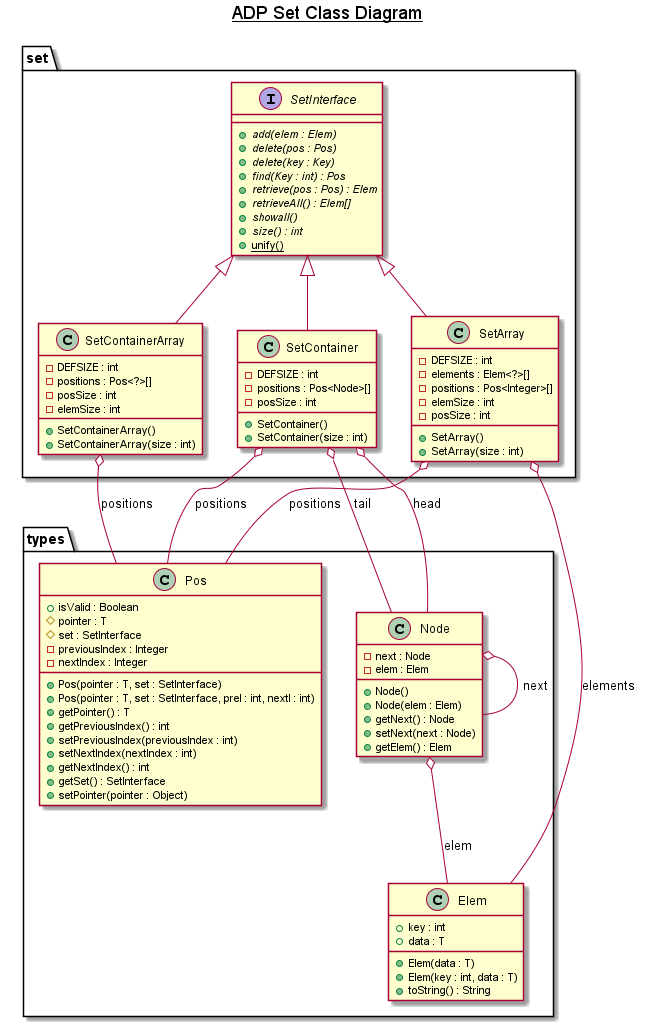
\includegraphics[width=\textwidth,height=\textheight,keepaspectratio]{BTI-ADP-SS19.png}
\caption{Klassendiagramm}
\label{figure:classdia}
\end{figure}

\subsection{Set als Array}
\label{sec:setArray}

Das Set wurde zunächst als Array implementiert. Hierfür wurde ein Array von der Elem-Klasse erstellt, sowie von der Pos-Klasse mit Zeigern auf die Integer-Indexe von Elem[].\\
Werden Plätze für Elemente im Set benötigt, so erfolgt eine dynamische Erstellung von Pos-Objekten, die die belegten und unbelegten Plätze im Set verwalten.\\
Beim Aufrufen der delete(Pos)-Methode werden jegliche Referenzen des Elements entfernt und Pos wird über isValid=FALSE unbelegt und später wieder beim Hinzufügen von Elementen benutzt.\\
Die Methode find(Key) iteriert die Positionen von der höchsten an und sucht dabei nach dem zugehörigen Element. Wird es nicht gefunden, so wird das invalide Stopper-Element als Position zurückgegeben.\\

\subsection{Set als Array von Containern}
\label{sec:setConArray}

Für die Implementation einer Menge mithilfe eines Arrays von Container-Klassen wurde die Container-Klasse Pos mit einem nextIndex und previousIndex versehen, 
welche auf den Integer-Index der vorherigen und nächsten Pos-Objekte im Container-Array zeigen. 
Hiermit wird eine stets korrekte Reihenfolge der Elemente im Set ermöglicht und sie ist realisiert durch folgende Mechaniken in den Methoden:\\
Wird ein neuer Pos-Container benötigt, dann wird er hinter den letzten Pos-Container durch setzen der Indexe angereiht.\\
In Abbildung \ref{figure:delmech} sieht man, wie beim Löschen eines Elements die laut nextIndex und previousIndex benachbarten Container durch ändern derer Indexe verknüpft werden. Der nun leere Container wird hinter den letzten Container in der Reihe eingereiht.
\begin{figure}[h!]
\texttt{ \\
// Link neighbours\\
int pre = positions[i].getPreviousIndex();\\
int next = positions[i].getNextIndex();\\
positions[pre].setNextIndex(next);\\
positions[next].setPreviousIndex(pre);\\
\\
// Append at ending\\
positions[positions[0].getPreviousIndex()].setNextIndex(i);\\
positions[i].setNextIndex(0);\\
positions[0].setPreviousIndex(i);\\
elemSize--;\\
}
\caption{Ausschnitt Lösch-Mechanik Container-Array}
\label{figure:delmech}
\end{figure}

Die Suche nach Elementen fängt von dem letzten Container in der Reihe an und läuft über previousIndex maximal bis zur Position von einem Stopper-Element, wo die Suche spätestens endet. Dies ist in Abbildung \ref{figure:findmech} zu sehen.\\
Die delete(Pos)-Methode iteriert auf die gleiche Weise.
\begin{figure}[h!]
\texttt{ \\
// Index 0 is reserved for stopper, but previousIndex always pointing to last Pos-Container in row\\
int i=0;    \\
while(true) {\\
    counter++;\\
    int pre = positions[i].getPreviousIndex();\\
    Elem tmp = (Elem)positions[pre].getPointer();\\
    if (tmp != null) {\\
        if (tmp.key == key) {\\
            return positions[pre];\\
        }\\
    } else {\\
        //error\\
        return null;\\
    }\\
    i = pre;\\
}\\
}
\caption{Ausschnitt Such-Mechanik Container-Array}
\label{figure:findmech}
\end{figure}

\subsection{Set als einfach verkettete Liste von Containern}
\label{sec:setCon}

Für die Implementation einer Menge mittels Container-Klassen wurde eine neue Klasse 'Node' erstellt. Diese Klasse hat einen Zeiger auf eine nächste Node, aber auch einen Zeiger auf ein Listenelement. Zusätzlich gibt es noch ein Pos-Array, dessen Pos auf Nodes zeigen.\\
Bei der Methode add(), wird zuerst mittels der Methode find(Key) überprüft, ob sich das Element schon in der Liste befindet und wenn nicht, welches Pos im Array als erstes frei ist, bzw. ob ein neues erstellt werden muss, welches dann auf die Node mit dem Element zeigt. Anschließend wird die Referenz des Pos mit dem neuen Element zurückgegeben.\\
Bei der Methode delete() wird die Pos von dem Element gesucht und anhand dieser, wird die Referenz der vorherigen Node auf die nachfolgende gesetzt. Bei der Pos wird isValid=false gesetzt.\\
Bei der Methode find() werden alle Nodes durchlaufen bis das Element gefunden wurde und anschließend die dazugehörige Pos gesucht und zurückgegeben.\\
Bei der Methode retrieve() wird das Pos-Array so lange durchsucht, bis wir die Pos die wir suchen gefunden haben und dann wird ihr Element zurückgegeben.\\

\section{Verifizieren und Testen}
\label{sec:vertests}

\subsection{Verifizieren der Funktionalität}
\label{sec:verfun}
Da die drei Varianten sich nur intern im Aufbau unterscheiden und dies nach außen hin gekapselt ist, verifizieren wir ihre Funktion anhand einer Menge an gleichen Tests.
Die in Tabelle ~\ref{table:vertests} enthaltenen Tests sollen eine ausreichende Verifizierung der Operationen auf den Sets ermöglichen.

\begin{table}
\begin{tabular}[ht]{|l|p{12cm}|}
\hline
T1             & \(add : SET \times ELEMENT \to SET \times POS\) \\ \hline
Beschreibung  & Hinzufügen eines Elements \(e \in ELEM\) in die Menge \(s \in SET\)           \\ \hline
pre-condition  & -           \\ \hline
post-condition & \texttt{s.find(e.key).isValid = TRUE}           \\ \hline
\hline
T2             & \(delete : SET \times POS \to SET\) \\ \hline
Beschreibung  & Entfernen eines Elements \(e \in ELEM\) in Position \(p \in POS\) aus der Menge \(s \in SET\)           \\ \hline
pre-condition  & \texttt{p.getSet() == s \&\& s.retrieve(p) == e \&\& p.isValid = TRUE}            \\ \hline
post-condition & \texttt{p.isValid = FALSE}           \\ \hline
\hline
T3             & \(delete : SET \times KEY \to SET\) \\ \hline
Beschreibung  & Entfernen eines Elements \(e \in ELEM\) in Position \(p \in POS\) mit Schlüssel \(k \in KEY\) aus der Menge \(s \in SET\)           \\ \hline
pre-condition  & \texttt{s.find(k).getSet() == s \&\& s.retrieve(s.find(k)) == e \&\& s.find(k).isValid = TRUE}            \\ \hline
post-condition & \texttt{p.isValid = FALSE}           \\ \hline
\hline
T4             & \(find : SET \times KEY \to POS\) \\ \hline
Beschreibung  & Suchen der Position \(p \in POS\) eines Elements \(e \in ELEM\) mit Schlüssel \(k \in KEY\) aus der Menge \(s \in SET\)           \\ \hline
pre-condition  & -           \\ \hline
post-condition & Wenn \(k \in s\): \texttt{s.find(k).isValid = TRUE}. Wenn \(k \notin s\): \texttt{s.find(k).isValid = FALSE}           \\ \hline
\hline
T5             & \(retrieve : SET \times POS \to ELEM\) \\ \hline
Beschreibung  & Zugriff auf Element \(e \in ELEM\) in Position \(p \in POS\) aus der Menge \(s \in SET\)           \\ \hline
pre-condition  & \texttt{p.getSet() == s \&\& p.isValid = TRUE}           \\ \hline
post-condition & \texttt{s.retrieve(p) == e}           \\ \hline
\hline
T6             & \(size : SET \to INTEGER\) \\ \hline
Beschreibung  & Mächtigkeit der Menge \(s \in SET\)           \\ \hline
pre-condition  & -           \\ \hline
post-condition & \texttt{s.size() == |s|}           \\ \hline
\hline
T7             & \(unify : SET \times SET \to SET\) \\ \hline
Beschreibung  & Vereinigung zweier Mengen \(s_{1},s_{2} \in SET\)           \\ \hline
pre-condition  & -           \\ \hline
post-condition & \texttt{s.unify(s1, s2) == }\(s_{1} \cup s_{2}\)           \\ \hline
\end{tabular}
\caption{Verifikationstests}
\label{table:vertests}
\end{table}

Die in der Tabelle ~\ref{table:vertests} aufgeführten Tests wurden mit verschiedenen Parametern und Quantitäten in verschiedenen Sequenzen in JUnit4 getestet. 
Alle drei Implementations-Varianten erfüllen die oben genannten Tests mit pre- und post-condition.

\subsection{Aufwandsanalyse}
\label{sec:aufwand}

Anhand der Tests und deren Ergebnisse, die in Abbildung 3.1, 3.2 und 3.3 visualisiert sind, ist sichtbar, dass delete mittels Pos immer effizienter ist als mittels Key. Dies ist dadurch erklärt, dass delete mittels Key zuerst die Pos des Elements finden muss und dann delete mittels Pos aufruft. Es ist auch sichtbar, dass die Implementation mit Array und Container in Arrays die selbe Effizienz haben und die Implementation mit Container in einer Liste weniger effizient ist, also die anderen beiden.

\begin{figure}
\newcommand{\bestCol}{brown}
\newcommand{\avgCol}{blue}
\newcommand{\worstCol}{red}
\newcommand{\posMark}{square*}
\newcommand{\keyMark}{*}
\begin{tikzpicture}
\begin{loglogaxis}[
	title={\large Array Test-Diagramm},
	height=15cm,
	width=15cm,
	grid=major,
    x tick label style={
        /pgf/number format/1000 sep=},
    ylabel=Operationen,
    xlabel=Listengröße,
    enlargelimits=0.05,
    legend style={at={(0.5,-0.1)},
    anchor=north,legend columns=-1},
]
\addplot[color=\bestCol,mark=\keyMark]
    coordinates {(100000,2) (10000,2)
         (1000,2) (100,2) (10, 2)};
\addplot[color=\avgCol,mark=\keyMark]
    coordinates {(100000,100000) (10000,10000)
         (1000,1000) (100,100) (10, 10)};
\addplot[color=\worstCol,mark=\keyMark]
    coordinates {(100000,200000) (10000,20000)
         (1000,2000) (100,200) (10, 20)};
\addplot[color=\bestCol,mark=\posMark]
    coordinates {(100000,1) (10000,1)
         (1000,1) (100,1) (10, 1)};
\addplot[color=\avgCol,mark=\posMark]
    coordinates {(100000,50000) (10000,5000)
         (1000,500) (100,50) (10, 5)};
\addplot[color=\worstCol,mark=\posMark]
    coordinates {(100000,100000) (10000,10000)
         (1000,1000) (100,100) (10, 10)};
\legend{KeyBest,KeyAverage, KeyWorst, 
PosBest,PosAverage, PosWorst}
\end{loglogaxis}
\end{tikzpicture}
\caption{delete(Pos) und delete(Key) in Array}
\end{figure}

\begin{figure}
\newcommand{\bestCol}{brown}
\newcommand{\avgCol}{blue}
\newcommand{\worstCol}{red}
\newcommand{\posMark}{square*}
\newcommand{\keyMark}{*}
\begin{tikzpicture}
\begin{loglogaxis}[
	title={\large ContainerArray Test-Diagramm},
	height=15cm,
	width=15cm,
	grid=major,
    x tick label style={
        /pgf/number format/1000 sep=},
    ylabel=Operationen,
    xlabel=Listengröße,
    enlargelimits=0.05,
    legend style={at={(0.5,-0.1)},
    anchor=north,legend columns=-1},
]
\addplot[color=\bestCol,mark=\keyMark]
    coordinates {(100000,2) (10000,2)
         (1000,2) (100,2) (10, 2)};
\addplot[color=\avgCol,mark=\keyMark]
    coordinates {(100000,100000) (10000,10000)
         (1000,1000) (100,100) (10, 10)};
\addplot[color=\worstCol,mark=\keyMark]
    coordinates {(100000,200000) (10000,20000)
         (1000,2000) (100,200) (10, 20)};
\addplot[color=\bestCol,mark=\posMark]
    coordinates {(100000,1) (10000,1)
         (1000,1) (100,1) (10, 1)};
\addplot[color=\avgCol,mark=\posMark]
    coordinates {(100000,50000) (10000,5000)
         (1000,500) (100,50) (10, 5)};
\addplot[color=\worstCol,mark=\posMark]
    coordinates {(100000,100000) (10000,10000)
         (1000,1000) (100,100) (10, 10)};
\legend{KeyBest,KeyAverage, KeyWorst, 
PosBest,PosAverage, PosWorst}
\end{loglogaxis}
\end{tikzpicture}
\caption{delete(Pos) und delete(Key) in Container-Array}
\end{figure}

\begin{figure}
\newcommand{\bestCol}{brown}
\newcommand{\avgCol}{blue}
\newcommand{\worstCol}{red}
\newcommand{\posMark}{square*}
\newcommand{\keyMark}{*}
\begin{tikzpicture}
\begin{loglogaxis}[
	title={\large Container Test-Diagramm},
	height=15cm,
	width=15cm,
	grid=major,
    x tick label style={
        /pgf/number format/1000 sep=},
    ylabel=Operationen,
    xlabel=Listengröße,
    enlargelimits=0.05,
    legend style={at={(0.5,-0.1)},
    anchor=north,legend columns=-1},
]
\addplot[color=\bestCol,mark=\keyMark]
    coordinates {(100000,4) (10000,4)
         (1000,4) (100,4) (10, 4)};
\addplot[color=\avgCol,mark=\keyMark]
    coordinates {(100000,150004) (10000,15004)
         (1000,1504) (100,154) (10, 19)};
\addplot[color=\worstCol,mark=\keyMark]
    coordinates {(100000,300001) (10000,30001)
         (1000,3001) (100,301) (10, 31)};
\addplot[color=\bestCol,mark=\posMark]
    coordinates {(100000,2) (10000,2)
         (1000,2) (100,2) (10, 2)};
\addplot[color=\avgCol,mark=\posMark]
    coordinates {(100000,100002) (10000,10002)
         (1000,1002) (100,102) (10, 12)};
\addplot[color=\worstCol,mark=\posMark]
    coordinates {(100000,200000) (10000,20000)
         (1000,2000) (100,200) (10, 20)};
\legend{KeyBest,KeyAverage, KeyWorst, 
PosBest,PosAverage, PosWorst}
\end{loglogaxis}
\end{tikzpicture}
\caption{delete(Pos) und delete(Key) in Container-Liste}
\end{figure}

\end{document}


%%% Local Variables:
%%% mode: latex
%%% TeX-master: t
%%% End:
